\documentclass{sigchi}
\usepackage{autobreak}
\usepackage{booktabs}
\usepackage{multirow}
\newcommand\tabhead[1]{\small\textbf{#1}}
\makeatletter
\def\@copyrightspace{\relax}
\makeatother


% Use this command to override the default ACM copyright statement (e.g. for preprints). 
% Consult the conference website for the camera-ready copyright statement.


%% EXAMPLE BEGIN -- HOW TO OVERRIDE THE DEFAULT COPYRIGHT STRIP -- (July 22, 2013 - Paul Baumann)
% \toappear{Permission to make digital or hard copies of all or part of this work for personal or classroom use is 	granted without fee provided that copies are not made or distributed for profit or commercial advantage and that copies bear this notice and the full citation on the first page. Copyrights for components of this work owned by others than ACM must be honored. Abstracting with credit is permitted. To copy otherwise, or republish, to post on servers or to redistribute to lists, requires prior specific permission and/or a fee. Request permissions from permissions@acm.org. \\
% {\emph{CHI'14}}, April 26--May 1, 2014, Toronto, Canada. \\
% Copyright \copyright~2014 ACM ISBN/14/04...\$15.00. \\
% DOI string from ACM form confirmation}
%% EXAMPLE END -- HOW TO OVERRIDE THE DEFAULT COPYRIGHT STRIP -- (July 22, 2013 - Paul Baumann)


% Arabic page numbers for submission. 
% Remove this line to eliminate page numbers for the camera ready copy
% \pagenumbering{arabic}


% Load basic packages
\usepackage{balance}  % to better equalize the last page
\usepackage{graphics} % for EPS, load graphicx instead
\usepackage{times}    % comment if you want LaTeX's default font
\usepackage{url}      % llt: nicely formatted URLs

% llt: Define a global style for URLs, rather that the default one
\makeatletter
\def\url@leostyle{%
  \@ifundefined{selectfont}{\def\UrlFont{\sf}}{\def\UrlFont{\small\bf\ttfamily}}}
\makeatother
\urlstyle{leo}


% To make various LaTeX processors do the right thing with page size.
\def\pprw{8.5in}
\def\pprh{11in}
\special{papersize=\pprw,\pprh}
\setlength{\paperwidth}{\pprw}
\setlength{\paperheight}{\pprh}
\setlength{\pdfpagewidth}{\pprw}
\setlength{\pdfpageheight}{\pprh}

% Make sure hyperref comes last of your loaded packages, 
% to give it a fighting chance of not being over-written, 
% since its job is to redefine many LaTeX commands.
\usepackage[pdftex]{hyperref}
\hypersetup{
pdftitle={Research on indoor positioning technology based on iBeacon},
pdfauthor={Shanliang Yao},
pdfkeywords={indoor positioning, iBeacon, Triangle Algorithm, Weighted Trilateration Algorithm},
bookmarksnumbered,
pdfstartview={FitH},
colorlinks,
citecolor=black,
filecolor=black,
linkcolor=black,
urlcolor=black,
breaklinks=true,
}

% create a shortcut to typeset table headings
\newcommand\tabhead[1]{\small\textbf{#1}}


% End of preamble. Here it comes the document.
\begin{document}

\title{Research on indoor positioning technology based on iBeacon}

\numberofauthors{1}
\author{
  \alignauthor Shanliang Yao\\
    \affaddr{Xi'an Jiaotong Liverpool University}\\
    \email{shanliang.yao19@student.xjtlu.edu.cn}\\
    \affaddr{+86 18896581232}
}

\maketitle

\begin{abstract}
Nowadays, some specific locations have troubled people when they look for their destinations. For example, when people are in an unfamiliar underground garage, they may get trapped when looking for their cars because there is no GPS signal. The practicability and necessity of indoor positioning in some specific occasions have become increasingly significant.

iBeacon is a new type of precision indoor micro-positioning technology based on Bluetooth 4.0. Currently, iOS and Android system devices all have Bluetooth Low Energy Technology (BLE) \cite{gomez2012overview}. In practice, there are multiple algorithms to obtain a relatively accurate position. In this research, I compare Trilateration Algorithm to Weighted Trilateration Algorithm and analyze the calculated coordinates and distances after several experiments. As a result, the Weighted Trilateration Algorithm achieves 79.17\% accuracy of the indoor positioning which is better than the Trilateration Algorithm. 

\textbf{keywords}: indoor positioning, iBeacon, Triangle Algorithm, Weighted Trilateration Algorithm
\end{abstract}

\section{Introduction}

\subsection{Background}

Numerous mobile applications (APP) are currently making use of positioning technologies such as the Global Positioning System (GPS) \cite{misra2006global}, which could detect the position information of the users. However, due to the signal attenuation caused by the construction materials of buildings or undergrounds, positioning systems cannot rely on GPS.

Bluetooth is a wireless technology standard for exchanging data over short distances. It has also been used for indoor positioning since it is a cost-effective and easy-to-deploy solution \cite{heydon2012bluetooth}. With the progress and development of telecommunication technologies, a recently proposed technology called iBeacon is widely adopted in many applications.

iBeacon is an emerging technology in the field of indoor positioning that has shown better performance compared to others. It is a set of protocols that can be used in indoor positioning systems by Apple. The protocols indicate that a new low-power, low-cost signal transmitter can be detected by nearby handheld electronic devices. When your device is close to an iBeacon base station, the device can sense the iBeacon signal (UUID and RSSI) \cite{feldmann2003indoor}, ranging from a few millimeters to 50 meters. This technology allows smartphones or other devices to execute commands within the sensing range of an iBeacon base station.

\subsection{Motivation}
I used to develop an application that can push advertisements when a customer arrives at a store for a mall. It also used the technology of indoor positioning based on iBeacon. However, the effect is not very satisfactory due to the fluctuation of the signal.
 
Now, I want to further study the technologies and algorithms of indoor positioning to choose the appropriate algorithm so that it can be used in the next applications. Moreover, with the rapid increase of data services and multimedia services, the demand for positioning and navigation is increasing. I want to study deeply in this field and make my own contributions.

\subsection{Problem Statement}

\subsubsection{Research Problems}
The Bluetooth positioning system estimates the distance between the target and the node through RSSI, and then calculates the position of the target. However, it is a big error to estimate the distance between the target and the node through RSSI. The previous literature shows that the main reasons are:

1). The underlying protocol of Bluetooth will automatically adjust the transmit power according to the needs.

2). The multipath effect exists in the indoor environment. \cite{liu2007survey}.

\begin{figure}[!h]
\centering
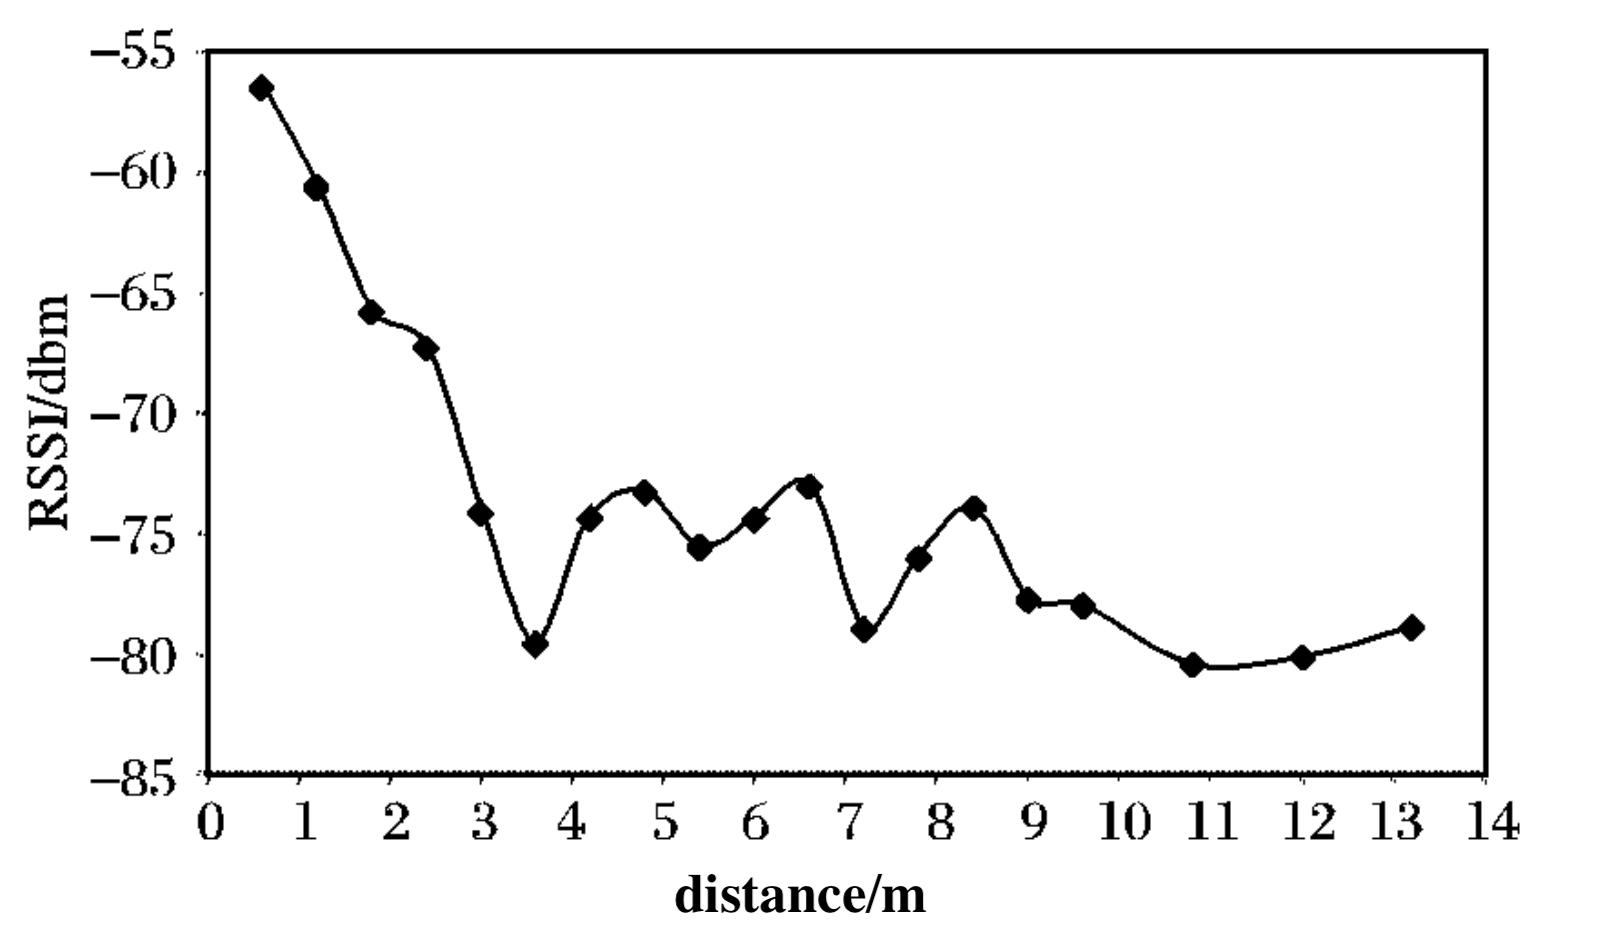
\includegraphics[width=1\columnwidth]{3.png}
\caption{Relationship between RSSI and distance}
\label{fig:universe}
\end{figure}


The measured relationship between the RSSI and the distance of the Bluetooth signal is shown in Figure 1. When the distance between the target and the node exceeds a certain range, the signal strength no longer decreases monotonically with the distance.

Thus, it is of significant important to deal with the problem with effective algorithms. When having solved this problem, indoor positioning will become more accurate.

\subsubsection{Research questions}

As the accuracy of indoor position has some problems, my research questions will be addressed: What algorithm can be used to improve the accuracy of indoor positioning?

By reading numbers of literature, I find that some algorithms need to be done to calculate the distance and the Trilateration Algorithm and the Weighted Trilateration Algorithm may be the best solution, Taking the two main algorithms into consideration, I put forward a hypothesis that compared with the Trilateration Algorithm, the Weighted Trilateration Algorithm can improve the accuracy of indoor positioning.

\subsubsection{Aims and Objectives}

The aim of this research is to test whether the Weighted Trilateration Algorithm is better than the Trilateration Algorithm.
Quantitative methods are used to gain in-depth insight into the accuracy of indoor positioning based on iBeacon. This data are analyzed and presented in the form of tables and charts.


\section{Literature Review}

This chapter first reviews different technologies in the field of indoor positioning. Then, it elaborates on the iBeacon technology. After that, it studies some algorithms about the indoor position. And finally, by summarizing all, it identifies and pins down some key issues that need to be addressed in the present study.

\subsection{Indoor Positioning Technology}

Indoor positioning has emerged as a critical function in many applications: including indoor personnel guidance, equipment guidance, security monitoring, property security and smart factories. From the journal \emph{Global Positioning System: signals, measurements and performance second edition} \cite{alarifi2016ultra}, it tell us that in comparison with outdoor environments, sensing location information in indoor environments requires a higher precision and is a more challenging task in part because various objects reflect and disperse signals . 

Technologies of indoor positioning vary, like Radio Frequency Identification (RFID), Ultra Wideband (UWB), Infrared (IR), Ultrasonic, Zigbee, Wireless Local Area Network (WLAN), Cellular Based, Bluetooth \cite{mautz2012indoor}. 

\subsection{iBeacon Technology}

In the World Wide Developers Conference (WWDC) 2013 event, Apple announced iBeacon, a technology that enables a device (called beacon) to send push notifications to nearby iOS devices \cite{conte2014bluesentinel}. The iBeacon is Apple's implementation of BLE wireless technology to create a different way of providing location-based information services to mobile devices. It acts as an emitter continuously broadcasting Bluetooth signals, in which each signal contains a Universally Unique Identifier (UUID) and a Received Signal Strength Indicator (RSSI).

This technology has significant advantages compared to other types of indoor positioning technologies, in its less expensive hardware, less energy consumption, needless to the internet connection, and is capable of receiving notifications in the background. This technology will provide huge benefits for future location awareness applications. It will change the way retailers, event organizers, and educational institutions communicate with people indoors \cite{fard2015indoor}. 

\subsection{Indoor Positioning Algorithms}

At present, there are various indoor positioning algorithms on the market which based on the principle of acquiring the signal strength of the surrounding Bluetooth base station through phones or other devices, such as Kalman Filter Algorithm, Gaussian Filtering Algorithm, Trilateration Algorithm and Weighted Trilateration Algorithm. In this research, I select Weighted Trilateration Algorithm and conduct experiments to compare it with the Trilateration Algorithm as both of them are the excellent algorithms and need to be researched more to discover the differences.

\subsubsection{Trilateration Algorithm}

In the ranging-based positioning algorithm, the Trilateration Algorithm \cite{liu2018trilateration} is a basic algorithm. The algorithm principle is: there are three non-collinear base stations A, B, C, and an unknown device D on the plane. The distance from the base station to the device D is R1, R2, and R3, and the coordinates of the three base stations are the center of the circle. The distance from the three base stations to the unknown device can be drawn as three intersecting circles, as shown in the following Figure 2.

\begin{figure}[h]
\centering
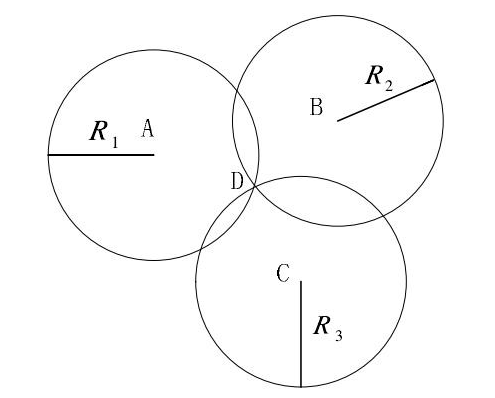
\includegraphics[width=0.7\columnwidth]{1}
\caption{Schematic diagram of the Trilateration Algorithm}
\label{fig:universe}
\end{figure}

Assume that there are n nodes randomly distributed in the wireless sensor network, and their location information is known: $(x_{1}, y_{1})(x_{2}, y_{2})(x_{3}, y_{3}) … (x_{n}, y_{n})$. Assume that the location information of the target node is X $(x_{T1}, y_{T1})$. So, the distance from the target node to each known node is:

\begin{equation*} 
d_{i}=\sqrt{(x_{T1}-x_{i})^{2}+(y_{T1}-y_{i})^{2}} \tag{1} 
\end{equation*}

Take the known node as the center and the radius from the known node to the target node as the radius. In theory, the intersection of the three circles is the coordinates of the target far point.

The Trilateration Algorithm formula is:

\begin{equation*} \begin{cases} (x_{T1}-x_{A})^{2}+(y_{T1}-y_{A})^{2}=d_{A}^{2}\\ (x_{T1}-x_{B})^{2}+(y_{T1}-y_{B})^{2}=d_{B}^{2}\\ (x_{T1}-x_{C})^{2}+(y_{T1}-y_{C})^{2}=d_{C}^{2} \end{cases} \tag{2} \end{equation*}

Through the transformation of the above formula, the coordinate information of the target node can be directly obtained as X $(x_{T1}, y_{T1})$:

\begin{equation} \begin{split} \begin{bmatrix} x_{T1}\\ y_{T1} \end{bmatrix}=\begin{bmatrix} 2(x_{A} -x_{C}) & 2(y_{A} -y_{C})\\ 2(x_{B}-x_{C}) & 2(y_{B}-y_{C}) \end{bmatrix}^{-1}
\\
\begin{bmatrix} x^{2}_{A}-x^{2}_{C}+y_{A}^{2}-y_{C}^{2}+d^{2}_{C}-d^{2}_{A}\\ x^{2}_{B}-x^{2}_{C}+y_{B}^{2}-y_{C}^{2}+d^{2}_{C}-d^{2}_{B} \end{bmatrix} \end{split} \tag{3}  \end{equation}


\subsubsection{Weighted Trilateration Algorithm}
However, in actual measurement, the three circles do not intersect at one point due to the measurement error, but intersect in a region. As a result, the Weighted Trilateration Algorithm is raised, as shown in the following Figure 3. 

\begin{figure}[!h]
\centering
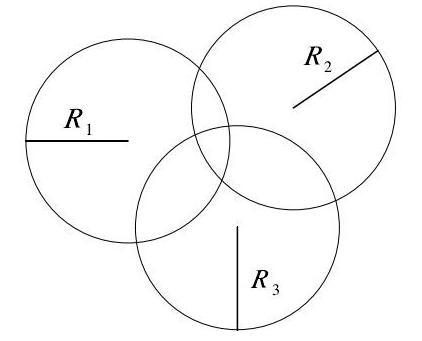
\includegraphics[width=0.6\columnwidth]{2}
\caption{Schematic diagram of the Weighted Trilateration Algorithm}
\label{fig:universe}
\end{figure}

Then add a weight $w$ and an $\beta$ to Equation (2). so that we get the unique X $(x_{T2}, y_{T2})$. To make this wand $\beta$ fit a variety of situations, use the Minimum Generalized Error method to optimize $w$ and $\beta$. By changing the values of wand $\beta$, the value of the unique target node X $(x_{T2}, y_{T2})$ is obtained.

\begin{equation*} \begin{cases} (x_{T2}-x_{A})^{2}+(y_{T2}-y_{A})^{2}=w_{A}d_{A}^{2}+\beta_{A}\\ (x_{T2}-x_{B})^{2}+(y_{T2}-y_{B})^{2}=w_{B}d_{B}^{2}+\beta_{B}\\ (x_{T2}-x_{C})^{2}+(y_{T2}-y_{C})^{2}=w_{C}d_{C}^{2}+\beta_{C} \end{cases} \tag{4} \end{equation*}

\subsection{Summary}
While there has been much research on comparison between different technologies, few researchers have taken algorithms into consideration. 
In this research, I use an RSSI-based algorithm as the method because it is simple to obtain the RSSI data from iBeacon by phone devices.

With the researcher's full understanding in the algorithms and strong capability in writing executable programs to test the function and performance of the algorithms, this research own its feasibility.

 
\section{Methodology}

\subsection{Research Method}

I choose quantitative methods to conduct my experiments. The two different algorithms are the independent variables, and the result of the calculated coordinates are the independent variables. Extraneous variables are the lab space, the iBeacons, and devices. All of them need to be the same.

\subsection{Research Design}

\subsubsection{Research Architecture}

\begin{figure}[!h]
\centering
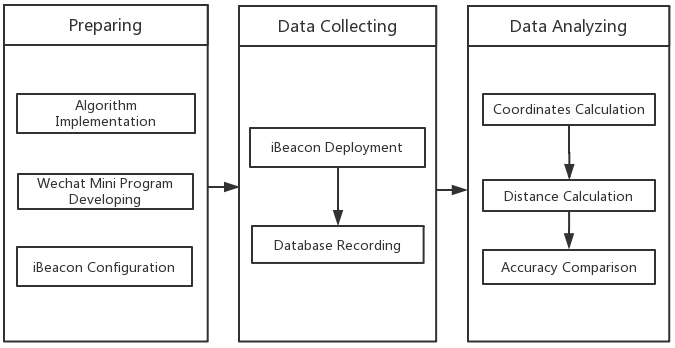
\includegraphics[width=1\columnwidth]{9.png}
\caption{Research Architecture}
\label{fig:9}
\end{figure}

As is described in Figure~\ref{fig:9}, first of all, two different algorithms need to be converted into executable code so that they can be applied in the real experiments. Besides, a wechat mini program is developed to test the result as it can provide the ability to use Bluetooth and can receive the RSSI and distance from the iBeacon. Then, I have configured 5 iBeacons on the parameters of uuid, major and minor for the program to test. After that, preparations are all done, and I begin to conduct the experiment and collect the data.

\subsubsection{Software for Collecting Data}

\begin{figure}[!h]
\centering
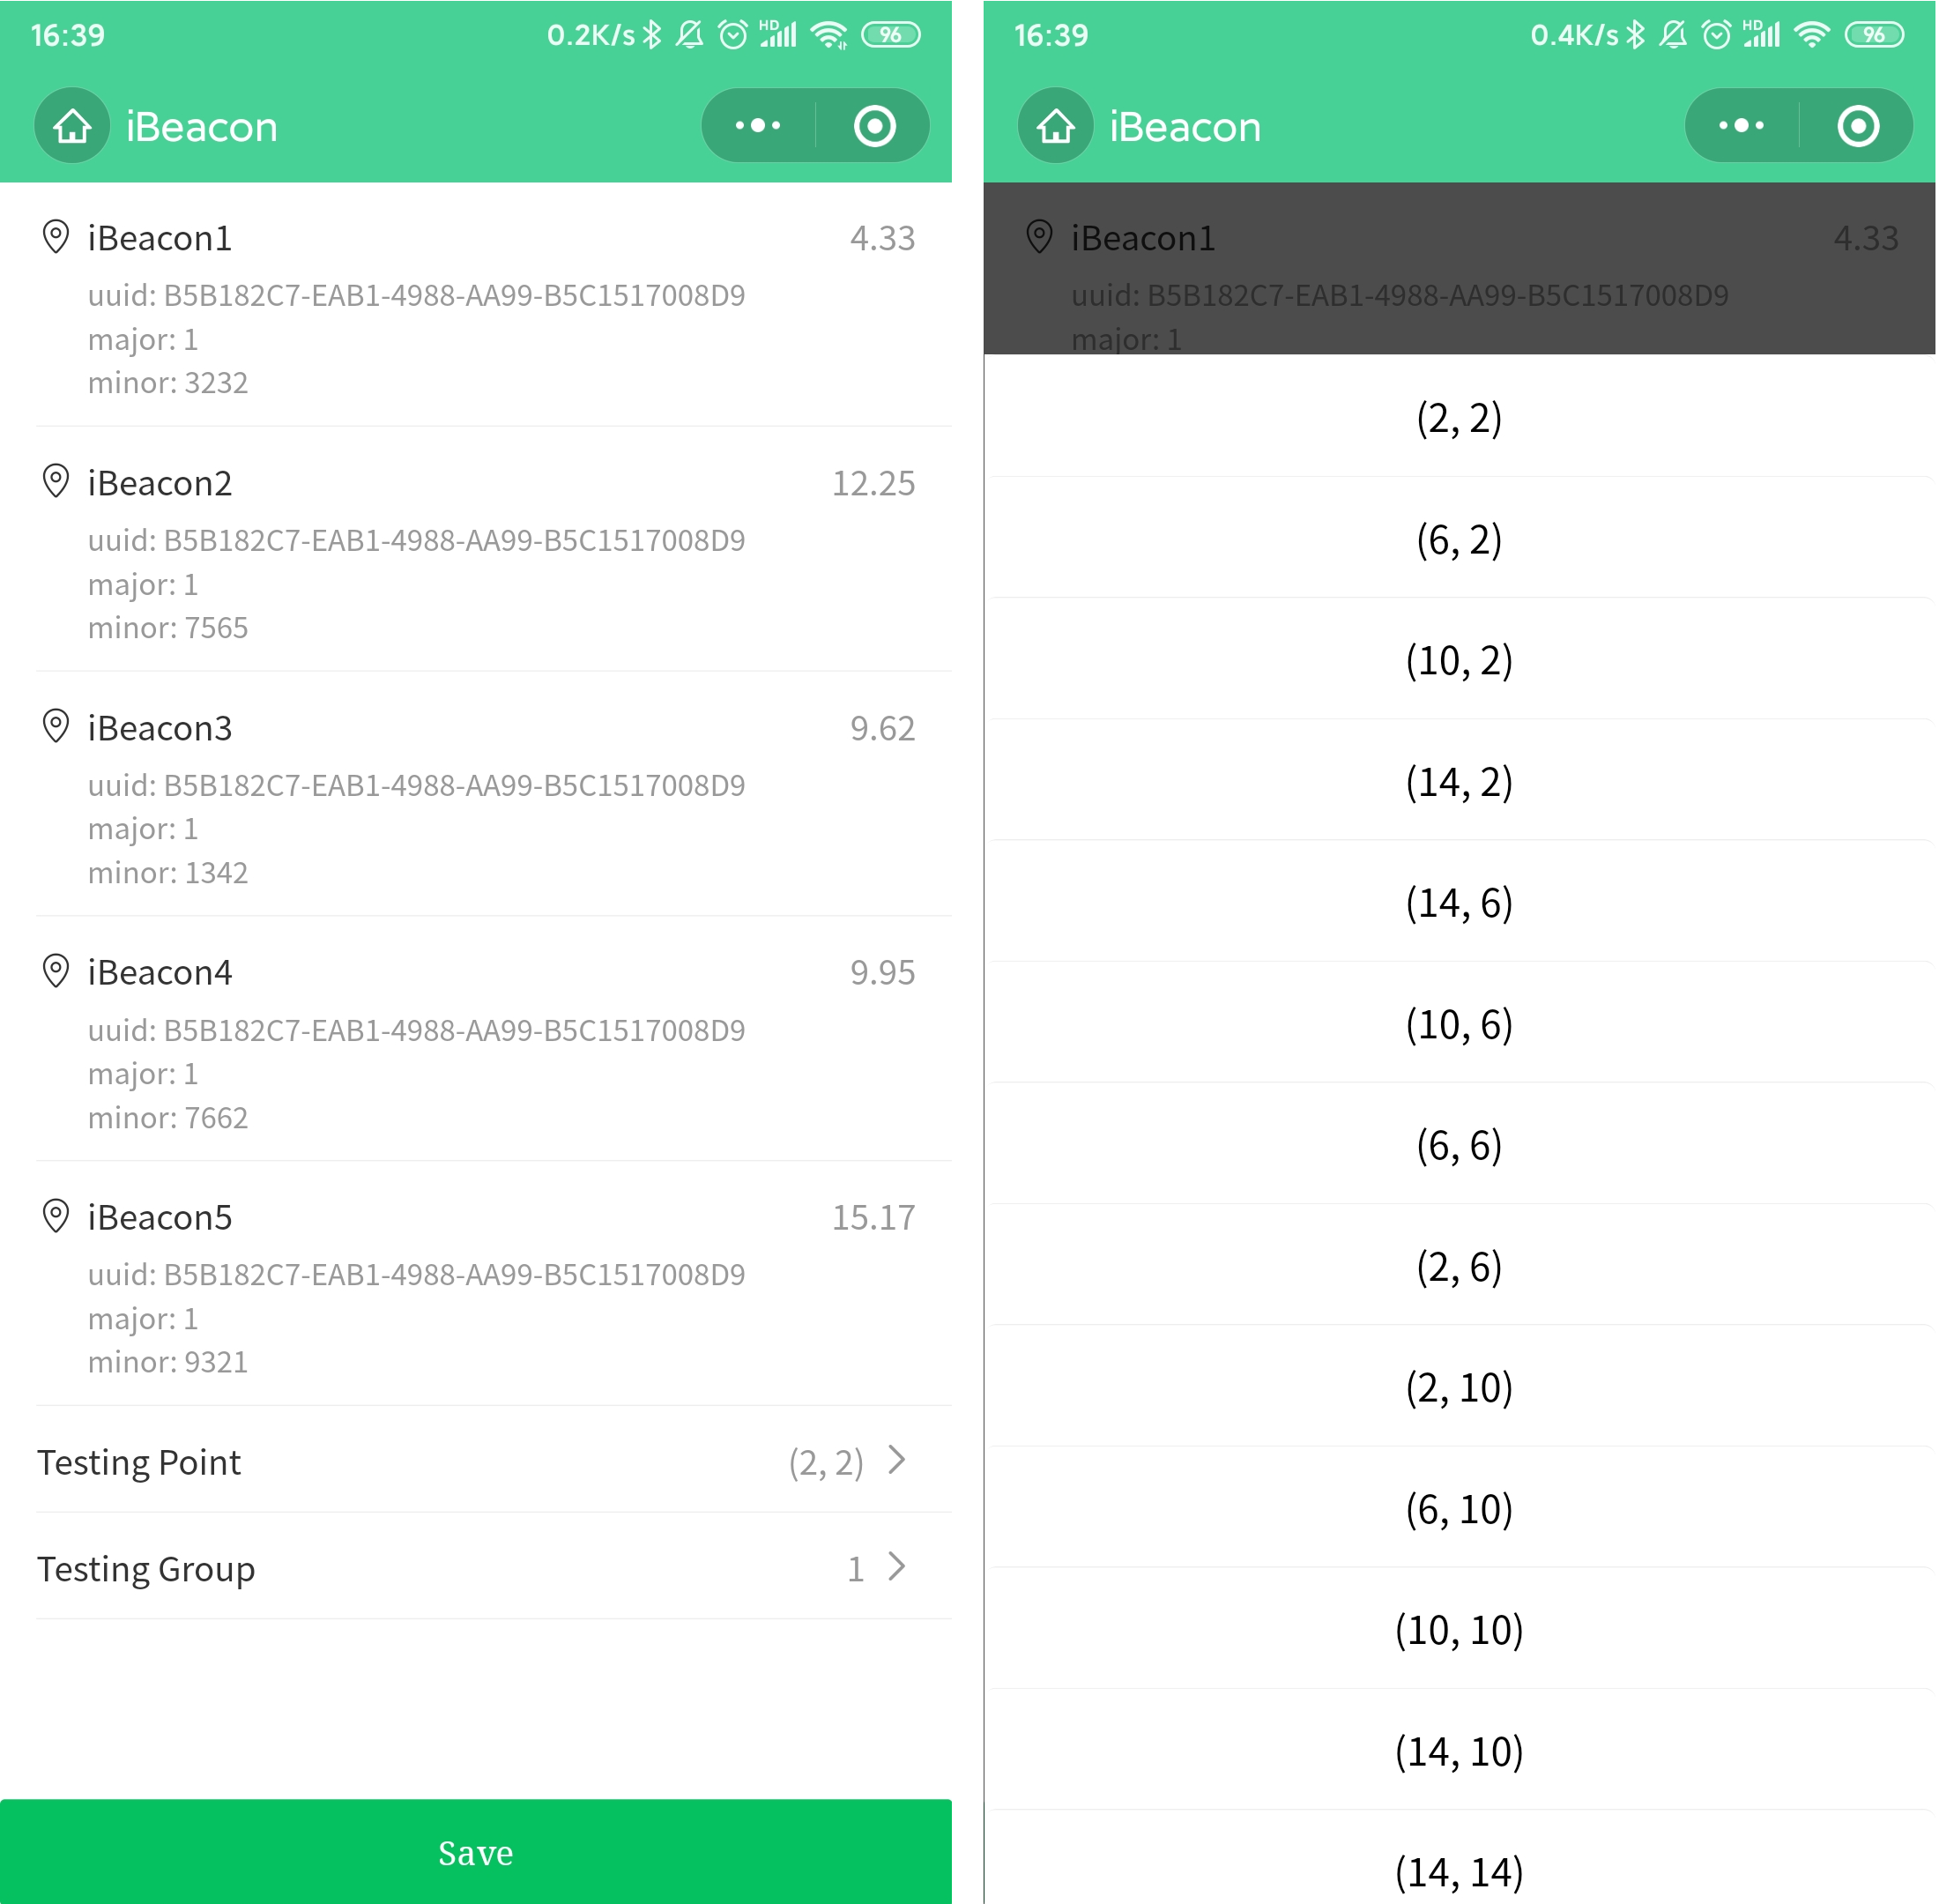
\includegraphics[width=1\columnwidth]{6.png}
\caption{Software for Collecting Data}
\label{fig:universe}
\end{figure}

To collect the data from iBeacons, I developed a software based on wechat mini program which is shown in Figure 5. The functions of this software are showing the information of each iBeacon including the distance and providing selection boxes to select the corresponding test group and coordinate position. At the bottom of the screen is a button to save the data to the database.

\subsubsection{Database for Storing Data}

\begin{figure}[!h]
\centering
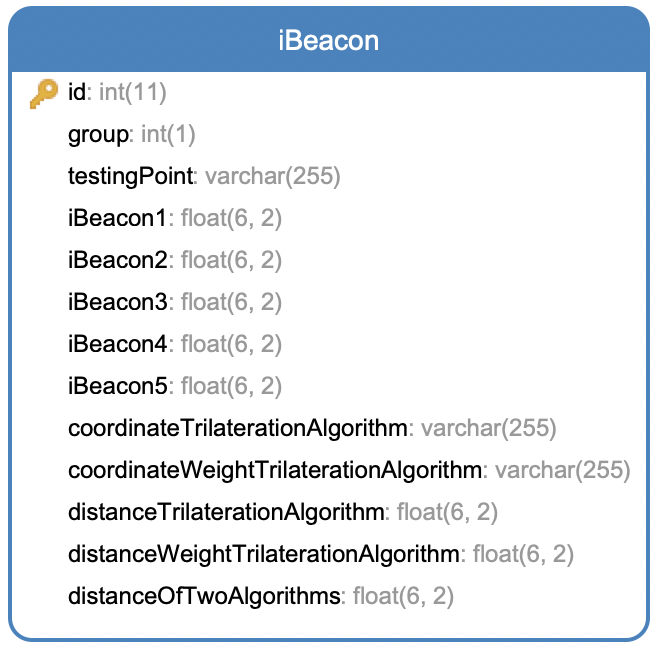
\includegraphics[width=1\columnwidth]{10.png}
\caption{Database of iBeacon for Storing Data}
\label{fig:universe}
\end{figure}

I have designed a database to store the data, the main table is the iBeacon for storing the distance of each iBeacon. As is shown in Figure 6, it contains several columns, like a coordinate of testing point, iBeacon1-5, coordinates of the two algorithms and distances of the two algorithms. At the beginning, it stores the information of each iBeacon. After the experiment, the columns of coordinate and distance are updated under the compared two algorithms.


\subsection{Experiment}

To evaluate the accuracy of the two algorithms, several experiments were conducted in the underground garage of the Science Building D (SD) at Xi'an Jiaotong-Liverpool University. The underground garage is shown in Figure 7.

\begin{figure}[!h]
\centering
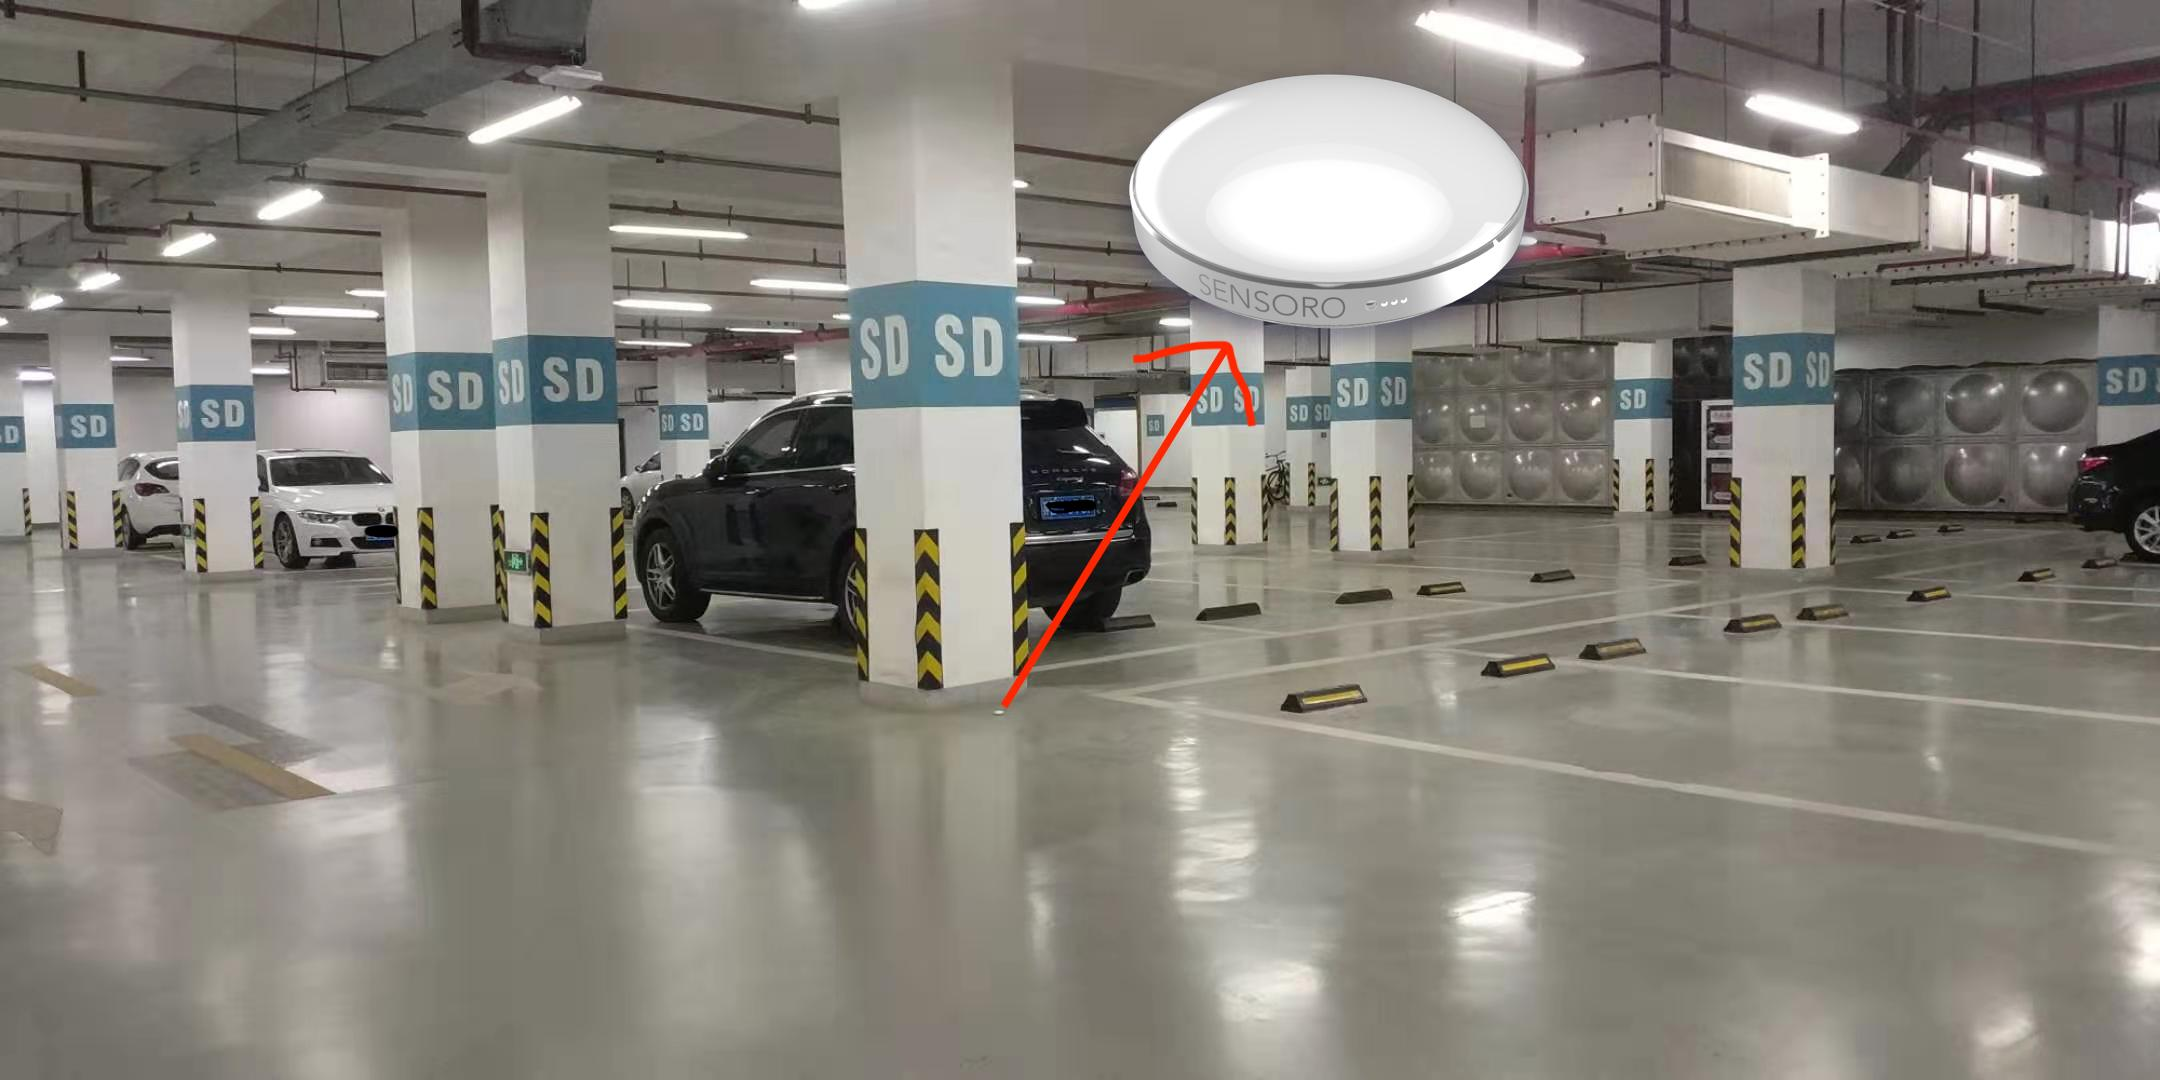
\includegraphics[width=1\columnwidth]{4.png}
\caption{Experiment environment: underground garage}
\label{fig:universe}
\end{figure}

\begin{figure}[!h]
\centering
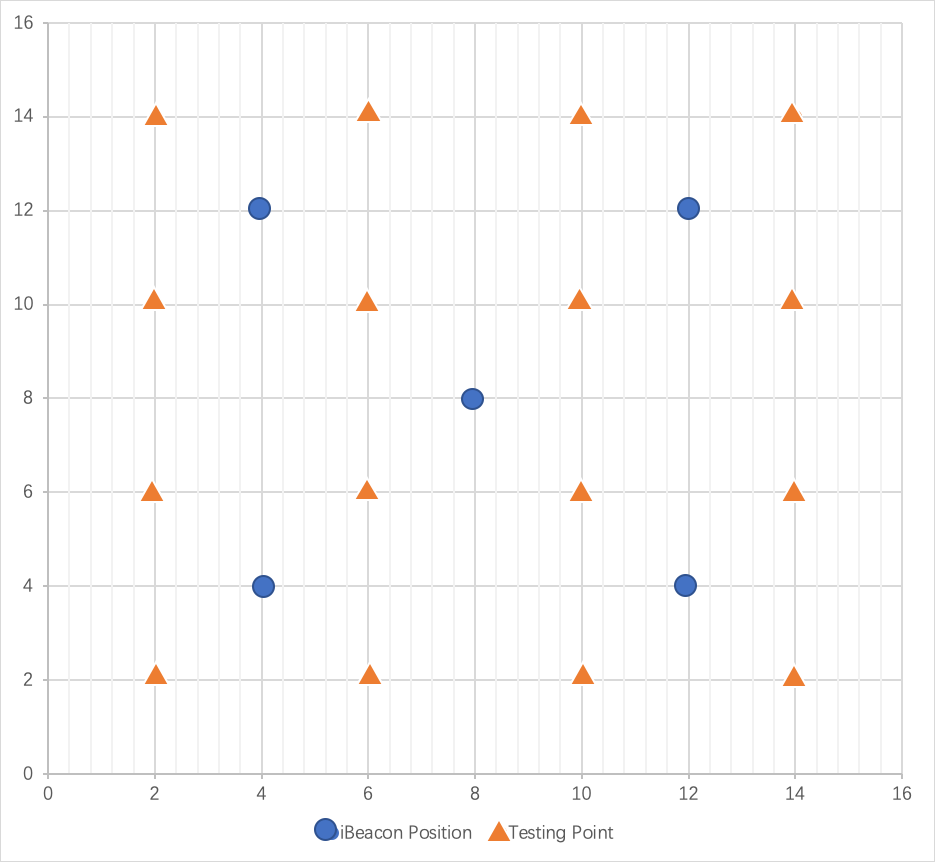
\includegraphics[width=1\columnwidth]{5.png}
\caption{Sketch map of the iBeacon position and testing point}
\label{fig:universe}
\end{figure}

As is vividly presented in Figure 8, the area I used is about 16Mx16M with 5 iBeacons deployed on designed points marked with blue circles on the map. Testing points are marked with range triangles around the iBeacons. 

The iBeacon used in this experiment is SENSORO which is widely used in the market. Besides, I used the Xiaomi MIX2 as the testing device, running Android version 9.

When testing the distance, I stood on each testing point for 3 seconds and then pressed the button on the wechat mini program to record the distance from each iBeacon. The program called an HTTP API offered by the server-side. 

\subsection{Data Collection}


\begin{table}[!h]
  \centering
  \begin{tabular}{|c|c|c|c|c|c|}
    \hline
    \tabhead {Testing Point} &
   \multicolumn{1}{|p{0.1\columnwidth}|}{\centering\tabhead{iBeacon 1 }} &
    \multicolumn{1}{|p{0.1\columnwidth}|}{\centering\tabhead{iBeacon 2 }} &
    \multicolumn{1}{|p{0.1\columnwidth}|}{\centering\tabhead{iBeacon 3 }} &
    \multicolumn{1}{|p{0.1\columnwidth}|}{\centering\tabhead{iBeacon 4 }} &
    \multicolumn{1}{|p{0.1\columnwidth}|}{\centering\tabhead{iBeacon 5 }} \\
    \hline
    (2, 2) & 4.33&12.25& 9.62& 9.95& 15.17 \\
    \hline
    (6, 2) & 3.74& 8.34& 8.45& 11.71& 13.88 \\
    \hline
    (10, 2) & 5.77 & 3.82 & 6.66 & 11.76 & 10.93 \\
    \hline
    (14, 2) & 7.8 & 1.28 & 6.41 & 12.03 & 9.24 \\
    \hline
    (14, 6) &9.69 & 1.69& 7.03& 12.65&8.3  \\
    \hline
    (10, 6) & 3.57& 4.63&3.16 &7.91 &8.44  \\
    \hline
    (6, 6) & 3.34&5.04 &2.93 &7.47 & 8.37 \\
    \hline
    (2, 6) &4.28 &8.71 & 3.61&7.91 &8.44  \\
    \hline
    (2, 10) &4.66 & 10.59& 5.66&4 &10.31  \\
    \hline
    (6, 10) & 8.29&9.78 &4.3 &2.32 & 5.68 \\
    \hline
    (10, 10) &7.36 &6.25 &1.73 &5.57 &3.98  \\
    \hline
    (14, 10) &12.44 &7.38 &6.95 & 10.31&2.46  \\
    \hline
    (14, 14) & 12.86& 9.43&7.21 &8.88 &1.6  \\
    \hline
    (10, 14) &13.06 &12.78 & 8.29&6.18 &5.55  \\
    \hline
    (6, 14) & 11.53& 13.81&8.34 &3.54 & 8.38 \\
    \hline
    (2, 14) & 10.32&13.65 &8.01 &2.48 &9.27  \\
    \hline
  \end{tabular}
  \caption{Some data of the experiment.}
  \label{tab:table1}
\end{table}

The wechat mini program collects the distance from deployed iBeacons. When testing the experiments, the values of distance report to the server and then store in the MySQL database in the form of key-value. I have conducted 3 groups of experiment and each group contains 16 testing points. It means that 48 points of data have been recorded for the later analysis. 

The above Table 1 shows one group data from the experiment. More data are presented in Appendix 1 Table 1.

\subsection{Data Analysis}
To compare the performances of the given two algorithms, the data of distance needed to be converted to the coordinate under the two algorithms. By passing the distance of the nearest 3 iBeacons into the two algorithms, I can get the coordinates under the corresponding algorithm.

The following Table 2 shows the result of the comparison. The first column is the real coordinate of the testing point {i} (called $(x_{Ti}, y_{Ti})$). The second column is the coordinate of testing point {i} under the Trilateration Algorithm (called $(x_{Ai}, y_{Ai})$). Also, the third column is the coordinate of testing point {i} under the Weighted Trilateration Algorithm (called $(x_{Bi}, y_{Bi})$).

\begin{table}[!h]
  \centering
  \begin{tabular}{|c|c|c|}
    \hline
    \tabhead{Testing Point} &
    \multicolumn{1}{|p{0.3\columnwidth}|}{\centering\tabhead{Trilateration Algorithm }} &
    \multicolumn{1}{|p{0.4\columnwidth}|}{\centering\tabhead{Weighted Trilateration Algorithm }} \\
    \hline
    (2, 2) & (-0.21, 2.99)&(0.24, 0.94) \\
    \hline
    (6, 2) & (4.53, 0.3)&(7.37, 3.13) \\
    \hline
    (10, 2) & (9.17, 1.44) & (11.77, 1.95)\\
    \hline
    (14, 2) & (11.7, 2.76) & (14.3, 3.52) \\
    \hline
    (14, 6) &(13.69, 3.87) & (14.39, 7.27)  \\
    \hline
    (10, 6) & (7.46, 4.89) & (10.58, 6.56)  \\
    \hline
    (6, 6) & (7.11, 5.21) & (4.53, 5) \\
    \hline
    (2, 6) &(4.4, 8.26) & (0.14, 6.62) \\
    \hline
    (2, 10) &(2.35, 8.36)&(0.96, 9.44)  \\
    \hline
    (6, 10) & (6.32, 11.96) & (5.21, 9.85) \\
    \hline
    (10, 10) &(8.95, 9.45) & (9.25, 8.63)  \\
    \hline
    (14, 10) &(14.26, 11.03) & (13.75, 8.41)  \\
    \hline
    (14, 14) & (12.77, 13.4) & (15.2, 12.29)  \\
    \hline
    (10, 14) &(8.46, 16.28)&(8.47, 13.59)  \\
    \hline
    (6, 14) & (4.39, 15.52)& (5.19, 15.3) \\
    \hline
    (2, 14) & (3.01, 14.27)&(1.57, 12.74) \\
    \hline
  \end{tabular}
  \caption{Coordinate of each testing point.}
  \label{tab:table1}
\end{table}

However, it’s not clear enough to look at the coordinates directly. Then, I calculated the distance between $(x_{Ai}, y_{Ai})$ and $(x_{Ti}, y_{Ti})$, and compared it with the distance between $(x_{Bi}, y_{Bi})$ and $(x_{Ti}, y_{Ti})$. In the following Table3, the second column means the distance (called D$_{Ai}$) between the testing point and the calculated coordinate under the Trilateration Algorithm. The third column means the distance (called D$_{Bi}$) between the testing point and the calculated coordinate under the Weighted Trilateration Algorithm. The fourth column is the difference between D$_{Ai}$ and D$_{Bi}$ which means that if the result is more than zero then the coordinate $(x_{Ai}, y_{Ai})$ is farther than the coordinate $(x_{Bi}, y_{Bi})$ compared with the real coordinate of the testing point $(x_{Ti}, y_{Ti})$.

\begin{table}[!h]
  \centering
  \begin{tabular}{|c|c|c|c|}
    \hline
    \tabhead{Testing Point} &
    \multicolumn{1}{|p{0.2\columnwidth}|}{\centering\tabhead{Trilateration Algorithm }} &
    \multicolumn{1}{|p{0.2\columnwidth}|}{\centering\tabhead{Weighted Trilateration Algorithm }} &
    \multicolumn{1}{|p{0.2\columnwidth}|}{\centering\tabhead{Distance }} \\
    \hline
    (2, 2) & 2.42&2.05&0.37 \\
    \hline
    (6, 2) & 2.25& 1.78&0.47 \\
    \hline
    (10, 2) & 1&1.77&-0.77\\
    \hline
    (14, 2) & 2.42&1.55&0.87 \\
    \hline
    (14, 6) &2.15&1.33&0.82  \\
    \hline
    (10, 6) & 2.77&0.81&1.96  \\
    \hline
    (6, 6) & 1.36&1.93&-0.57 \\
    \hline
    (2, 6) &3.3&1.96&1.34 \\
    \hline
    (2, 10) &1.68&1.18&0.5  \\
    \hline
    (6, 10) & 1.99& 0.8 & 1.99 \\
    \hline
    (10, 10) &1.19&1.56&-0.37  \\
    \hline
    (14, 10) &1.06&1.61&-0.55  \\
    \hline
    (14, 14) & 1.37&2.09&-0.72  \\
    \hline
    (10, 14) &2.75&1.58&1.17  \\
    \hline
    (6, 14) & 2.21&1.53&0.68 \\
    \hline
    (2, 14) & 1.05&1.33&-0.28 \\
    \hline
  \end{tabular}
  \caption{Distance from the testing point.}
  \label{tab:table1}
\end{table}

\section{Results}

To test and compare the performances of the given two algorithms, the accuracy (ACC) is adopted for evaluating the results. An accurate algorithm will have a higher ACC value. As is shown in the following Equation (5), the value of ACC is the sum of closer points divided by total points.

\begin{equation*} ACC(\%)=\frac{\text{Closer}\ \text{Points}}{\text{Total}\ \text{Points}}\% \tag{5} \end{equation*}

\begin{figure}[htbp]
\centering
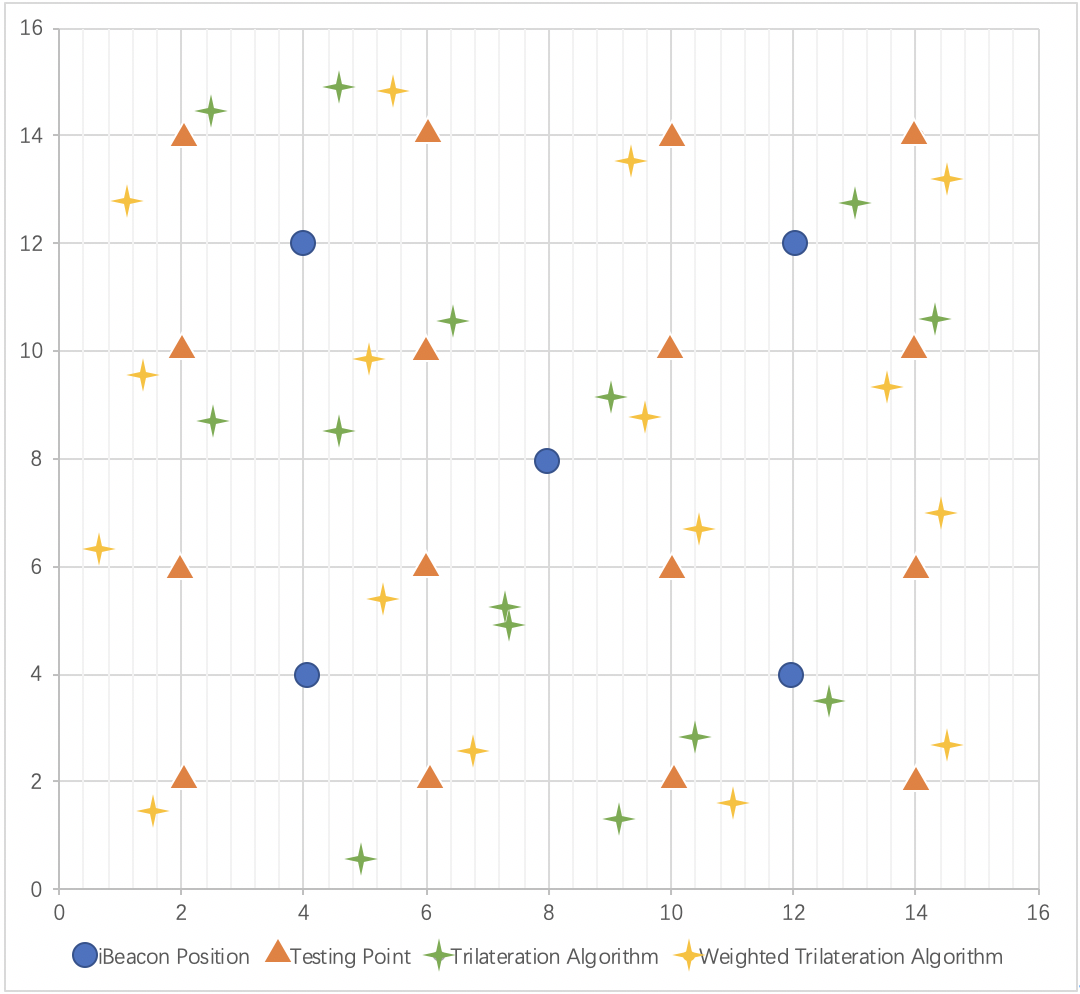
\includegraphics[width=1\columnwidth]{7.png}
\caption{Sketch map of the calculated coordinates}
\label{fig:universe}
\end{figure}

In this experiment, 38 testing points are closer to the testing point under the Weighted Trilateration Algorithm than under the Weighted Trilateration Algorithm. By passing that value and the number of total points into the equation, I can get the ACC of the Weighted Trilateration Algorithm is 79\%. It means that the Weighted Trilateration Algorithm gets better accuracy than the Trilateration Algorithm and just proves my hypothesis is correct.

To visually show the coordinate distribution calculated by the two algorithms, I mark each coordinate in the sketch map. It can be clearly seen that the yellow stars are closer to each testing point than the green stars.


\section{Discussion}
\subsection{Limitations}
The result shows that the Weighted Trilateration Algorithm gets better accuracy. However, there can be a different result that the Weighted Trilateration Algorithm is not as good as the Trilateration Algorithm.

Firstly, due to the limitation of iBeacon, I can only test one kind of iBeacon which can be sold in the market. More experiments need to be conducted by test different bands of iBeacon.

Secondly, due to the limitation of phone devices, other devices may get different RSSI and distance values. For further consideration, I will work on other experiments through different devices.

Thirdly, the average error of iBeacon is between 1 and 3 meters \cite{grzechca2016analysis}. However, due to the limitation of the experimental environment, the step interval of the experiment may cause data deviation. So a larger range of tests is needed to be conducted.

\subsection{Contributions}
In this paper, I aim to bridge the gap between the recent development in this area and the existing related survey by presenting a comparative survey of indoor positioning technologies and algorithms. Contributions in this research can be summarized as follows:

1). I provide updated research on existing indoor positioning technologies and algorithms that I believe would spur further exploration by the research community of this difficult problem area.

2). I provide a comparative analysis of indoor positioning technologies and algorithms to help indoor positioning developers in choosing the appropriate algorithms for their applications.

\section{Conclusion}

In the research, I have conducted research on the indoor positioning algorithm based on iBeacon. The result shows that the Weighted Trilateration Algorithm is better than the Trilateration Algorithm in its accuracy in 79\% of the cases which can help people reach their destinations.

Besides, I have developed a software for collecting the RSSI and distances of the iBeacons. Moreover, data analysis methods are effective and clear which can vividly and intuitively show the results. I would like to conduct further experiments and optimize the indoor position algorithm to improve the accuracy of indoor positioning.


% Balancing columns in a ref list is a bit of a pain because you
% either use a hack like flushend or balance, or manually insert
% a column break.  http://www.tex.ac.uk/cgi-bin/texfaq2html?label=balance
% multicols doesn't work because we're already in two-column mode,
% and flushend isn't awesome, so I choose balance.  See this
% for more info: http://cs.brown.edu/system/software/latex/doc/balance.pdf
%
% Note that in a perfect world balance wants to be in the first
% column of the last page.
%
% If balance doesn't work for you, you can remove that and
% hard-code a column break into the bbl file right before you
% submit:
%
% http://stackoverflow.com/questions/2149854/how-to-manually-equalize-columns-
% in-an-ieee-paper-if-using-bibtex
%
% Or, just remove \balance and give up on balancing the last page.
%
\balance

% REFERENCES FORMAT
% References must be the same font size as other body text.

% \bibliographystyle{acm-sigchi}
\bibliographystyle{unsrt}
\bibliography{sample}

\end{document}

